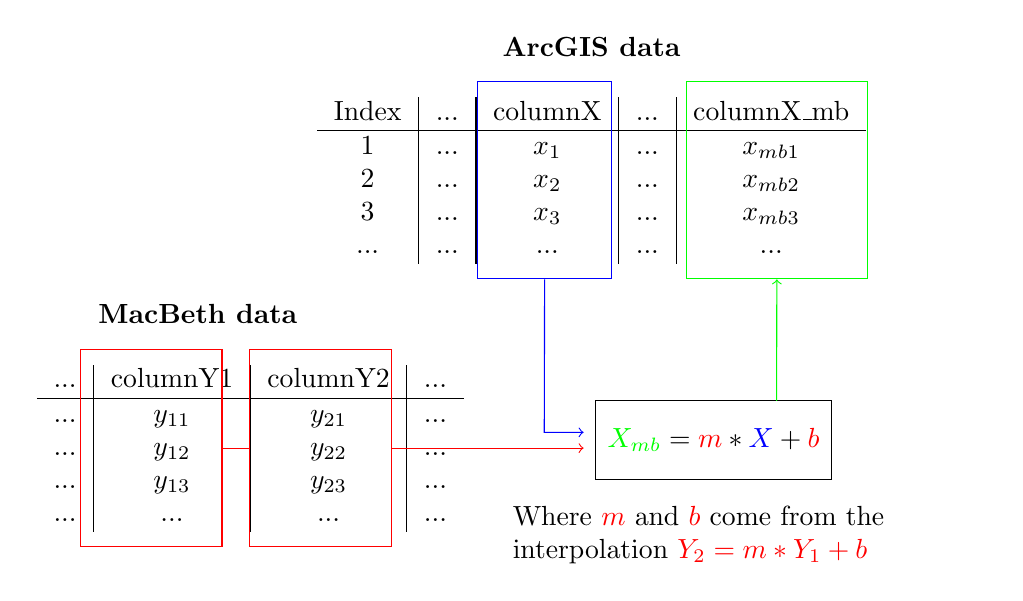
\begin{tikzpicture}
    % Tables
    \node (tab1) {%
        \begin{tabular}{c|c|c|c|c}
            Index  & ... & columnX & ... & columnX\_mb \\
            \hline
            1 & ... & $x_1$ & ... & $x_{mb1}$ \\
            2 & ... & $x_2$ & ... & $x_{mb2}$ \\
            3 & ... & $x_3$ & ... & $x_{mb3}$ \\
            ... & ... & ... & ... & ...
        \end{tabular}
    };
    \node [left,xshift=-1.5cm,yshift=-3.4cm] (tab2) {%
        \begin{tabular}{c|c|c|c}
            ... & columnY1 & columnY2 & ...\\
            \hline
            ... & $y_{11}$ & $y_{21}$ & ...\\
            ... & $y_{12}$ & $y_{22}$ & ...\\
            ... & $y_{13}$ & $y_{23}$ & ... \\
            ... & ... & ... & ...
        \end{tabular}
    };

    % Table labels
    \node[yshift=1.7cm] {\textbf{ArcGIS data}};
    \node[xshift=-5cm, yshift=-1.7cm] {\textbf{MacBeth data}};

    % Rectangles
    \node [
        rectangle,
        draw=blue,
        right,
        xshift=-1.45cm,
        minimum width=1.7cm,
        minimum height=2.5cm,
    ] (rec-x) {};
    \node [
        rectangle,
        draw=red,
        right,
        xshift=-6.5cm,
        yshift=-3.4cm,
        minimum width=1.8cm,
        minimum height=2.5cm,
    ] (rec-y1) {};
    \node [
        rectangle,
        draw=red,
        right,
        xshift=-4.35cm,
        yshift=-3.4cm,
        minimum width=1.8cm,
        minimum height=2.5cm,
    ] (rec-y2) {};
    \node [
        rectangle,
        draw=green,
        right,
        xshift=1.2cm,
        minimum width=2.3cm,
        minimum height=2.5cm,
    ] (rec-mb) {};
    \node [
        draw,
        rectangle,
        xshift=1.55cm,
        yshift=-3.3cm,
        minimum width=3cm,
        minimum height=1cm,
    ] (rec) {
        $\textcolor{green}{X_{mb}} = \textcolor{red}{m} * \textcolor{blue}{X} + \textcolor{red}{b}$
    };

    % Labels
    \node [xshift=2cm, yshift=-4.5cm, text width=6cm] {
        Where $\textcolor{red}{m}$ and $\textcolor{red}{b}$ come from the\\
        interpolation $\color{red} Y_2 = m * Y_1 + b$
    };

    % Arrows
    \draw [->, blue] (rec-x) -- (-0.6cm,-3.2cm) -- (-0.1cm,-3.2cm);
    \draw [-, red] (rec-y1) -- (rec-y2);
    \draw [->, red] (rec-y2) -- (-0.1cm,-3.4cm);
    \draw [->, green] (2.35cm,-2.8cm) -- (rec-mb);

\end{tikzpicture}